\documentclass{standalone}

\usepackage{graphicx}

\usepackage{tikz}

\usetikzlibrary{positioning}
\usetikzlibrary{arrows.meta}
\usetikzlibrary{calc}

\begin{document}

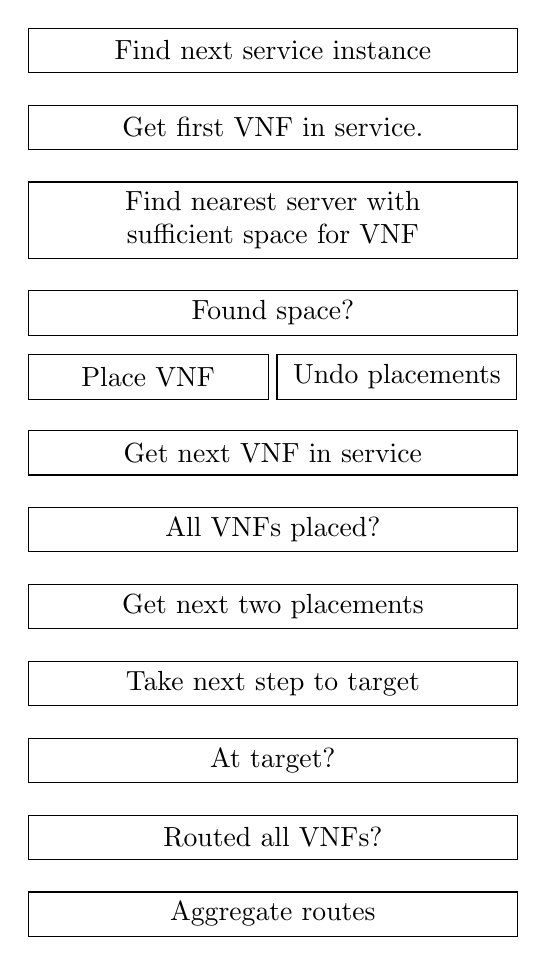
\begin{tikzpicture}[
    block/.style={align=center, rectangle, draw=black, fill=white, text width=17em, minimum height=1.6em},
    half/.style={align=center, rectangle, draw=black, fill=white, text width=8em, minimum height=1.6em}
]
    \node[block] (I1) [] {Find next service instance};

    \node[block] (P0) [below=0.4cm of I1] {Get first VNF in service.};
    \node[block] (P1) [below=0.4cm of P0] {Find nearest server with sufficient space for VNF};
    \node[block] (P2) [below=0.4cm of P1] {Found space?};

    \node (H1) [below=0.4cm of P2] {}; 
    \node[half] (P3) [left=-0.07cm of H1] {Place VNF};
    \node[half] (P4) [right=0.1cm of P3] {Undo placements};
    \node[block] (P5) [below=1.2cm of P2] {Get next VNF in service};

    \node[block] (P6) [below=0.4cm of P5] {All VNFs placed?};
    \node[block] (P7) [below=0.4cm of P6] {Get next two placements};
    \node[block] (P8) [below=0.4cm of P7] {Take next step to target};
    \node[block] (P9) [below=0.4cm of P8] {At target?};
    \node[block] (P10) [below=0.4cm of P9] {Routed all VNFs?};
    \node[block] (P11) [below=0.4cm of P10] {Aggregate routes};


    % \node[] (H1) [below=0.1cm of B8] {};
    % \node[] (H2) [right=0.7cm of B2] {};

    % \draw[-latex] (I1.south) -- (I2.north);
    % \draw[-latex] (I2.south) -- (B2.north);
    % \draw[-latex] (B2.south) -- (B3.north);
    % \draw[-latex] (B3.south) -- (B4.north);
    % \draw[-latex] (B4.south) -- (B5.north);
    % \draw[-latex] (B5.south) -- (B6.north);
    % \draw[-latex] (B6.south) -- (B7.north);
    % \draw[-latex] (B7.south) -- (B8.north);

    % \draw[-latex] (B8.south) -| (H1.south) -| (H2.west) -- (B2.east);

    % \draw[thick,dotted] ($(I1.north west)+(-1,0.8)$) rectangle ($(I2.south east)+(1.3,-.4)$);
    % \node[] at ($(I1.north west)+(0.4,0.45)$) {\textbf{Initialisation}};

    % \draw[thick,dotted] ($(B2.north west)+(-1,0.8)$) rectangle ($(B8.south east)+(1.3,-1)$);
    % \node[] at ($(B2.north west)+(0.4,0.45)$) {\textbf{Optimisation}};

    % \draw[thick,dotted] ($(B4.north west)+(-0.6,0.8)$) rectangle ($(B7.south east)+(0.3,-0.15)$);
    % \node[] at ($(B4.north west)+(0.4,0.45)$) {\textbf{In Parallel}};

\end{tikzpicture}

\end{document}